\section{Прямое произведение множеств, мощность прямого произведения конечных множеств. 
Бинарные отношения между множествами A и B. Граф бинарного отношения Матрица 
бинарного отношения, область определения и значений бинарного отношения. Отношение, 
обратное к данному отношению. Найти отношение, изобразить его граф, найти матрицу.}

Пусть $A$ и $B$ -- не пустые множества.
\begin{definition}
    \textit{Прямым (декартовым) произведением множеств $A$ и $B$}
    называют множество всевозможных упорядоченных пар $(a, b), a \in A, b \in B$.
    \begin{align*}
        A \times B = \set{(a,b) | a \in A, b \in B}
    \end{align*}
\end{definition}

Пример:
\begin{align*}
    A &= \set{1,2}, B=\set{a,b,c} \\
    A \times B &= \set{(1, a) , (1, b), (1, c), (2, a), (2, b), (2, c)} \\
    |A| &= n, |B| = m, |A \times B| = n \cdot m
\end{align*}

Если $A=B$, то пишут $A \times A = A^2$.

\begin{definition}
    \textit{Кортеж длины s} -- упорядоченный набор $(a_1,a_2,\dots,a_s)$, где $a \in A_i$.
    \begin{align*}
        A_1 \times A_2 \times \dots \times A_s = \set{(a_1,a_2,\dots,a_s), a_i \in A_i, i \in \overline{1,s}} \\
        |A_i| = t_i \\
        \text{Тогда: } |A_1 \times A_2 \times \dots \times A_s| = t_1 \cdot t_2 \cdot \dots \cdot t_s \\
        \text{Если: } A_1=A_2=\cdots=A_s=A, \text{ то пишут } A_1 \times A_2 \times \dots \times A_s = A^s
    \end{align*}
\end{definition}

\begin{definition}
    \textit{Бинарным отношение между множествами $A$ и $B$} называется
    любое подмножество их прямого произведения.
    Бинарные отношение принято записывать большими буквами или малыми буквами:
    \begin{align*}
        A&=\set{1,2},B=\set{a,b,c}\\
        R&=\set{(1,a),(2,b),(2,c)}\\
        f&=\set{(1,b),(2,a)}
    \end{align*}
    Если $(a,b) \in R$, то говорят, что элементы $a$ и $b$ связаные отношение $R$
    или находятся в отношении $R$. Обозначают: $aRb$.
\end{definition}

Сам граф бинарного отношения будет иметь вид:
\begin{figure}[h]
    \centering
    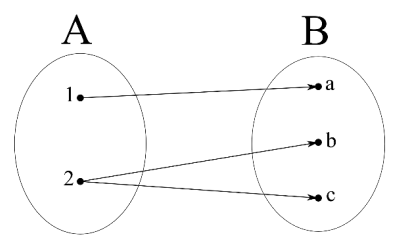
\includegraphics[scale=0.5]{6_grapg.png}
\end{figure}

Пусть бинарное отношение $R \subset A \times B, |A|=n, |B|=m$.
\begin{definition}
    \textit{Матрицой бинарного отношения R} называется матрица \mbox{$C(R) \in M_{n \times m}$},
    элементы которой находятся по правилу:
    \begin{align*}
        c_{ij}=\begin{cases}
        1, \text{ если } a_iRb_j \\
        0, \text{ иначе} 
        \end{cases}.
    \end{align*}
    Пример:
    \begin{align*}
        A&=\set{1,2}, B=\set{a,b,c} \\
        R&=\set{(1,a),(2,b),(2,c)} \\
        C(R)&=\begin{pmatrix}
            1 & 0 & 0 \\
            0 & 1 & 1
        \end{pmatrix}
    \end{align*}
\end{definition}

\begin{definition}
    \textit{Областью определения бинарного отношения $R$} называется
    множество первых элементов пар бинарного отношения.
    \begin{align*}
        D(R)=\set{x \in A | (\exists y \in B)(xRy)}
    \end{align*}
\end{definition}

\begin{definition}
    \textit{Областью значений бинарного отношения $R$} называется
    множество вторых элементов пар бинарного отношения.
    \begin{align*}
        E(R)=\set{y \in B | (\exists x \in A)(xRy)}
    \end{align*}
\end{definition}

Пример:
\begin{align*}
    A&=\set{1,2}, \; B=\set{a,b,c} \\
    R&=\set{(1,b),(2,c),(2,a),(2,b)} \\
    D(R)&=\set{1,2}, \; E(R)=\set{a,b,c}
\end{align*}

\begin{definition}
    \textit{Обратное бинарное отношение к $R$ ($R^{-1}$)} называется им,
    если: $$R^{-1}=\set{(y,x)|(x,y) \in R}$$
\end{definition}

Пример:
\begin{align*}
    R&=\set{(1,b),(2,c),(2,a),(2,b)} \\
    C(R)&=\begin{pmatrix}
        0 & 1 & 0 \\
        1 & 1 & 1
        \end{pmatrix} \\
    R^{-1}&=\set{(b,1),(c,2),(a,2),(b,2)} \\
    C(R)&=\begin{pmatrix}
        0 & 1 \\
        1 & 1 \\
        0 & 1
        \end{pmatrix}
\end{align*}
{
Заметим, что матрица $C(R^{-1})$ является транспонированной
матрицей $C(R)$.